\chapter{Analyse}

\section{Risiken}
Die vierte industrielle Revolution, das \ac{IIoT} und dessen Vielzahl an aktiven und passiven Elementen stellen in ihrer Komplexität eine große Herausforderung für die IT-Sicherheit dar. Einerseits muss die Sicherheit der laufenden Software, der Infrastruktur, Anwendungs- und Rechnersysteme gewährleistet werden, andererseits muss die Betriebssicherheit der Geräte und Anlagen, welche mit dem Internet verbunden sind sichergestellt werden. Das Management der IT-Sicherheit in Industrie 4.0 Netzen geht über Unternehmensgrenzen hinweg, da Netze und Systeme für Kunden, Lieferanden und Partner bereitgestellt werden \cite{DTAG2016}. Somit hat sich auch die Bedrohungslage der Netze geändert. Das \ac{BSI} beschreibt die Top 10 Bedrohungen und deren Folgen für \ac{ICS} \cite{ICSSec2016}.

\begin{enumerate}
    \item Social Engineering und Phishing - 
    \item Einschleusen von Schadsoftware über Wechseldatenträger und externe Hardware - 
    \item Infektion mit Schadsoftware über Internet und Intranet - 
    \item Einbruch über Fernwartungszugänge - 
    \item Menschliches Fehlverhalten und Sabotage - 
    \item Internet-verbundene Steuerungskomponenten - 
    \item Technisches Fehlverhalten und höhere Gewalt - 
    \item Kompromittierung von Extranet und Cloud Komponenten - 
    \item \ac{DoS} und \ac{DDoS} - 
    \item Kompromittierung von Smartphones im Produktionsumfeld - 
\end{enumerate}

Um die in \autoref{Grundlagen:Grundprinzipien der sicheren Kommunikation} genannten Schutzziele umzusetzen, ist es notwendig einen größtmöglichen Schutz gegen diese Bedrohungen bereitzustellen. Dafür müssen die Netzwerkinfrastruktur, Integrationsansätze und die eigentliche Kommunikation über die genutzten Protokolle gesichert werden. Dies geschieht u.a. durch die Abschottung von Systemen, die Einschränkung von Zugangsberechtigungen, die Härtung der Sicherheit der genutzten Komponenten, den Einsatz von Verschlüsselungsverfahren und die Schulung der Mitarbeiter um ein Sicherheitsbewusstsein zu schaffen und die Einhaltung von Sicherheitsrichtlinien zu gewährleisten.

\section{Netzwerkinfrastruktur}
heterogene Netze machen Probleme - Globale Netze haben Latenz, Paketverlust, usw.; müssen Anforderungen gerecht werden.

\subsection{Sicherheitsstrategien}
\subsubsection{Security by Design}
TODO - siehe DTAG2016 + Paulus

\subsubsection{Defense in Depth Strategie - TODO (Kuipers,2006)}

\begin{figure}[h]
    \centering
    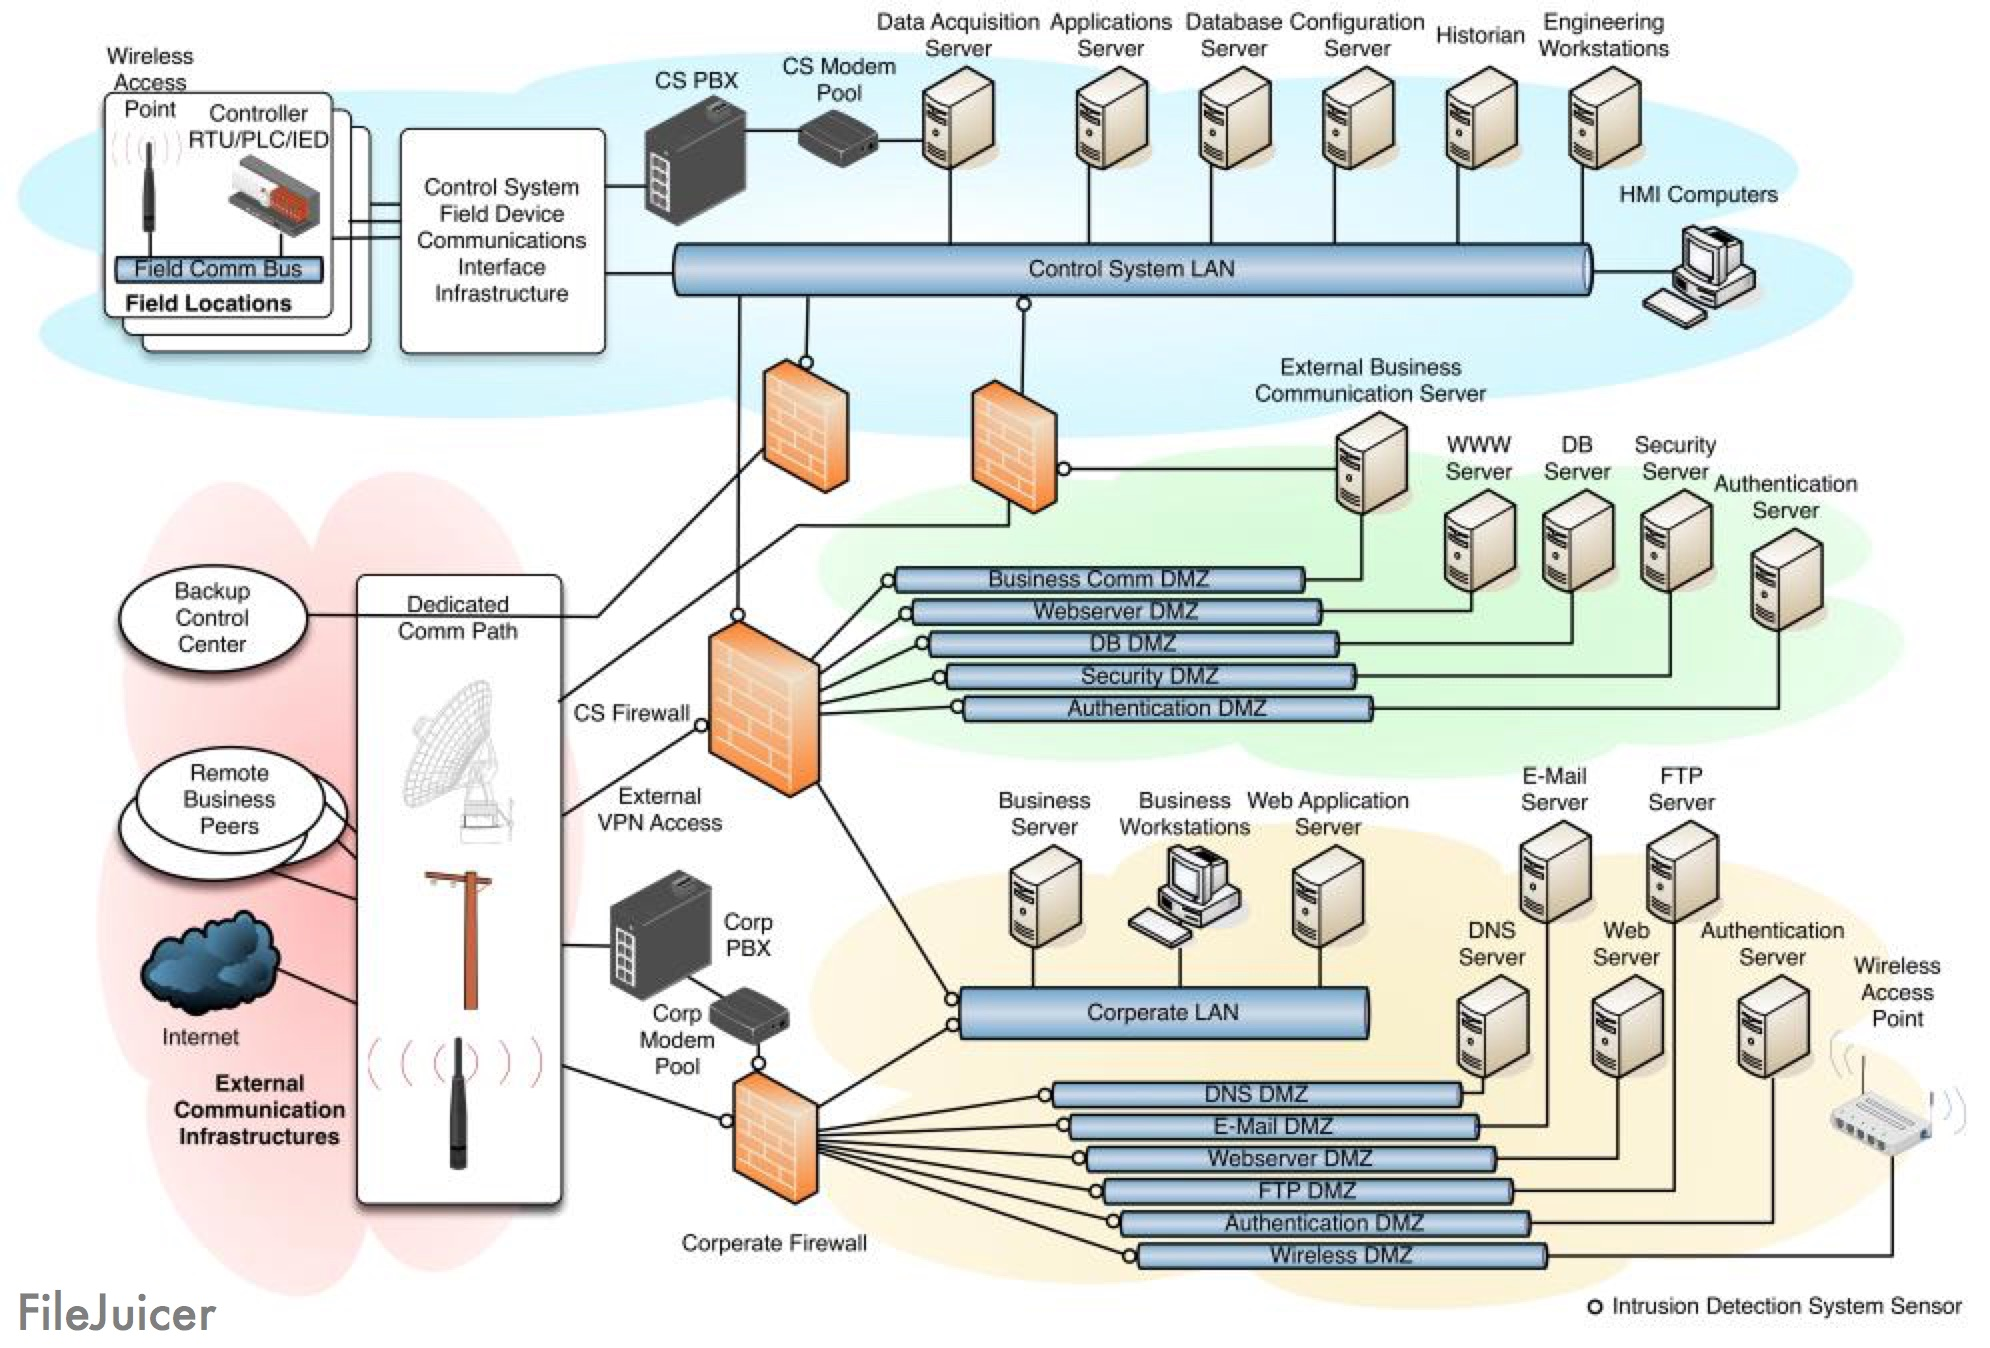
\includegraphics[width=15cm]{defense-in-depth-strategie}
    \caption{Defense in Depth Strategie - TODO ref. Kuipers,2006}
    \label{Kap3:Defense-in-Depth}
\end{figure}

\clearpage

TODO - Beschreibung und Einordnung der Defense in Depth Strategie

\subsection{Übertragungsmedium}
Als Übertragungsmedien können neben der klassischen Kabelverbindung auch andere (instabile) Kanäle wie Mobilfunk oder Satelliten in Frage kommen. Um die Kommunikation über alle Medien sicher und zuverlässig zu gestalten, müssen auf technischer Ebene Protokolle genutzt werden, welche es ermöglichen die gegebenen Schutzziele zu realisieren und die Integrität der Daten bei der Übertragung über große Entfernungen zu gewährleisten.

TODO - Übertragungsdistanz - Latenz - Jitter - usw.

\subsection{Integrationsansätze}
TODO - Probleme bei Migration alter Systeme - Inkompatibilität - spezielle bzw. proprietäre Protokolle - besondere Anforderungen der Shop-Floor-Ebene - Industrial Ethernet
TODO - MPLS -> schlecht

\subsubsection{Konsolidierung der Netzwerkkommunikation}
TODO - alles spricht OPC UA
Ansatz: Teuer, aufwendig bzw. nicht möglich, da embedded System bzw. keine Ressourcen oder keine Schnittstellen

\subsubsection{Gatewaykommunikation}
TODO - siehe Trumpf, axoom -> Gateways übersetzen von heterogener Netzwerkkommunikation in Protokollstandard für unternehmensübergreifende bzw. externe Kommunikation.
Ansatz: Softwareschwachstellen, Softwarefehler, müssen viele Herstellerprotokolle unterstützen - Probleme? - bekommt man Appliance zum Testen?

\section{Protokollanalyse}
\subsection{OPC UA}
\subsection{DDS}
\subsection{MQTT}
\subsection{CoAP}

\section{Angriffsvektoren}
\subsection{Verschlüsselung}
\subsection{Paketversand}
\subsection{TODO}

\section{Maßnahmenkatalog}

\subsection{TODO}

\section{Auswertung der Ergebnisse}
TODO - Grundlage der Implementierung!